\label{chpt:discussion} % for referencing this chapter elsewhere, use \ref{chpt:label}
\lhead{\emph{Discussion}} % This is for the header on each page - perhaps a shortened title

The analysis of this section includes eclipse modelled data from several sources: the 15 systems contained in this thesis, the 15 CVs characterised by \citet{McAllister2019}, and the 14 CVs modelled by \citet{Savoury2011}. A catalogue of all these data is given in Appendix~\ref{appendix:eclipse modelled CV data tables}. Note that there is some overlap between the data of \citet{McAllister2019} and \citet{Savoury2011}, and where this is the case the more recent findings of \citet{McAllister2019} are preferred.


\section{Three CVs with peculiar white dwarf colours}
\label{sect:discussion:three CVs with peculiar white dwarf colours}

All three systems were candidate post-period minimum systems based on their periods and preliminary eclipse data; none show a prominent bright spot (indicative of a low mass transfer rate), or significant donor flux (implying a dim donor).
As a result of this work, ASASSN-16kr and SSSJ0522-3505 are confirmed as having evolved through the period minimum and now have sub-stellar donors, and ASASSN-17jf lies in the period minimum region of Figure~\ref{fig:M2_vs_P}.
Additionally, all three white dwarf masses derived in this analysis fall within the range of CV white dwarf masses observed by \citet{pala2020}, of $\langle M_{\rm WD}\rangle = 0.83 \pm 0.17 M_\odot$, significantly higher than the pre-CV DA white dwarf mass of only $0.66 \pm 0.15 {\rm M_\odot}$ \citep{mccleery2020}.


\begin{figure*}
    \centering
    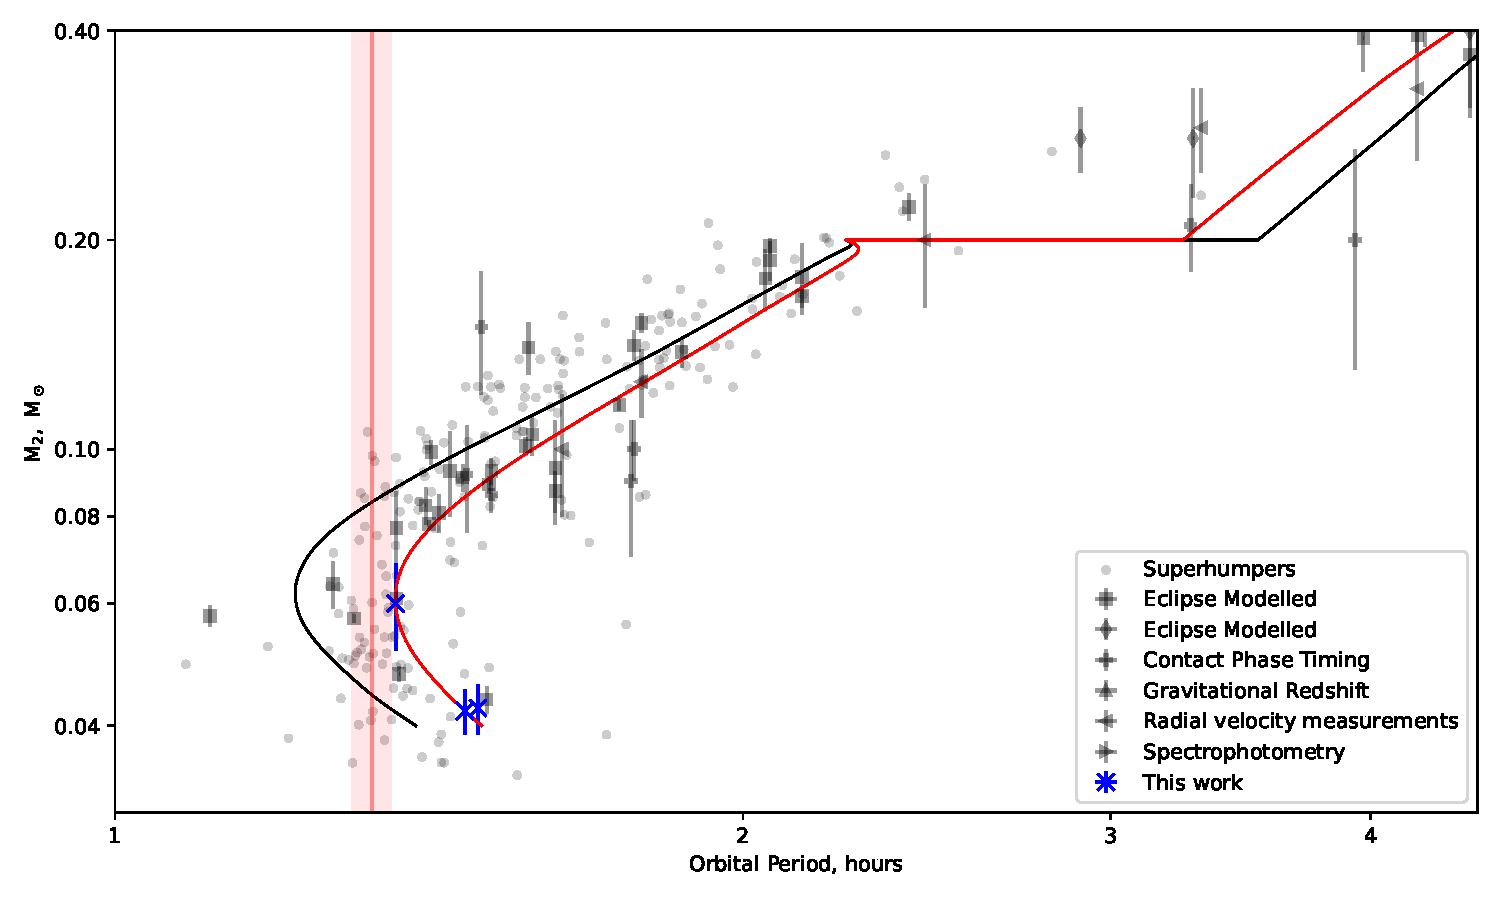
\includegraphics[width=\textwidth]{figures/results/three_cvs_with_weird_colours/GeneralFigs/M2_vs_P_withhumpers.pdf}
    \caption{Donor evolution tracks, from MESA modelling. The }
    \label{fig:M2_vs_P}
\end{figure*}

\subsection{Is it correct to assume an unobscured white dwarf?}
\label{sect:impure white dwarf discussion}

As discussed in \S\ref{sect:white dwarf temperature report}, the white dwarf colours may differ from model grids because the white dwarf ingress/egress is contaminated by an additional source of light, such as a boundary layer close to the surface.
If the eclipse is polluted by some other feature, phase-folded eclipse modelling will be wrong in two key elements: comparing colours to model atmospheres will be inaccurate, and the ingress and egress durations that constrain the white dwarf radius will not be correct.
\citet{Spark2015} conducted a study into the validity of assuming a pure white dwarf, comparing CV eclipse observations with white dwarfs with and without a few types of surface features such as boundary layers on the white dwarf, hot spots, or an optically thick or thin equatorial belt.
These features are revealed by a departure from symmetry between the white dwarf ingress and egress, but care must be taken not to confuse the flickering component of the CV with the signature of surface features.

Unfortunately, detecting a surface layer or hot spot on the white dwarf requires both a high time resolution and high signal-to-noise ratios. \citet{Spark2015} make use of SALTICAM data at a cadence of 0.15s, but the observations available here have a $\sim$3-4s exposure time and lower signal-to-noise. Measuring the eclipse precisely enough to make claims about the nature of the white dwarf's surface is therefore not possible with present observations.
The three systems of this work are prime candidates to search for WD eclipse asymmetries, as the issue of flickering corrupting the white dwarf ingress/egress derivative is largely mitigated; all three have little to no flickering present.
Future observations at higher cadence would open the possibility of examining the surfaces of these white dwarfs, though a large telescope will necessary due to the faintness of the systems; HiPERCAM on the GTC is an ideal candidate.


\subsection{The hot white dwarf of SSSJ0522-3505}
\label{sect:SSSJ0522-3505 white dwarf temperature discussion}

The effective temperature of white dwarfs in short period CVs is typically $\sim10000$K \citep{Pala2017a}, but the observed colours of SSSJ0522-3505 indicate a much hotter $T_{\rm eff}$ of $\sim25000$K. This is likely to be accurate, as the system's observations are clearly dominated by the white dwarf flux, and show roughly the same eclipse depth in the $r', g'$, and $u'$ bands, which would not be consistent with a lower white dwarf temperature.

The measured effective temperature could be wrong, either as a result of poor flux calibration (see \S\ref{sect:observations:flux calibrating the lightcurve} for reasons this is unlikely) or because the ingress/egress fluxes do not represent the fluxes of the white dwarf photosphere, as discussed in section~\ref{sect:impure white dwarf discussion}. However, the measured temperature is  $\sim10000$\,K hotter than expected, and these effects are unlikely to have introduced an error of this magnitude. As support for this, note that \citet{Pala2017a} find that white dwarf temperatures from UV spectroscopy typically agree with those measured from eclipse lightcurves to within $\sim1000$\,K. Reasons why the white dwarf temperature in SSSJ0522-3505 might be unusually hot are explored here, but UV spectroscopy to confirm the white dwarf temperature is highly desirable.

The white dwarf in a CV is thought to settle at an equilibrium temperature, where radiative heat loss is balanced with two energy sources: energy released by infalling material, and a low level of "simmering" nuclear fusion in the white dwarf envelope \citep{Townsley2003, Townsley2004}, but there are several reasons that this white dwarf may be temporarily out of equilibrium.
There is no reason, though it is unlikely, that a CV cannot form from a main sequence star with a brown dwarf companion, to produce a young CV with a low-mass donor and a white dwarf still cooling from its formation temperature.
Once the donor has reconnected with its Roche lobe, it would rejoin the normal CV evolution track and otherwise behave as a normal CV, with a normal accretion rate but a younger, hotter white dwarf than is typical.

A recent dwarf nova outburst was observed in this system in 2011, and could have produced a temporary boost to $T_{\rm eff}$. During these events, the disc enters a hot, optically thick state, and the infall rate onto the white dwarf is greatly increased \citep{osaki1996}, releasing a significant amount of energy and heating the white dwarf surface.
This is only the most recent \textit{observed} outburst, as there is a gap in observations between 2013 and 2019 during which any outburst events would have gone unrecorded. This may be important, as recent X-ray observations of another post period minimum system, OV Bootis \citep{Schwope2021}, shows that the WD temperature is increased to 23000K, 5 months after outburst, 9000K hotter than its $T_{\rm eff}$ prior to outburst. The increase in temperature can be somewhat long lasting; detailed observations of GW Lib have shown its WD is still 3000K hotter than equilibrium 8 years post-outburst\citep{Szkody2016}.
Another possibility is a recent classical nova -- thermonuclear runaway in an accreted surface layer on the white dwarf -- which would temporarily heat the white dwarf beyond its equilibrium temperature \citep{starrfield2016}, giving the impression of a hotter white dwarf than expected, though a classical nova resulting in such a strong heating effect would be surprising.

However, assuming the white dwarf is in thermal equilibrium, $T_{\rm eff}$ can be used to estimate the long-term accretion rate of the system \citep{townsley2009}.
If the modelled $T_{\rm eff}$ of SSSJ0522-3505 is both accurate and driven by accretion, it would correspond to $\dot M_{\rm WD} = 6\pm2 \times 10^{-10} M_\odot {\rm yr^{-1}}$, compared to accretion rates of $\sim10^{-10}-10^{-11} M_\odot {\rm yr^{-1}}$ expected for CVs in the post-period minimum regime \citep{Pala2017a}. Unfortunately, the MESA-based method to find $\dot M$ cannot be reliably applied to this system, as the $M_{\rm donor}$ is too low.
Whilst high, a mass accretion rate of $10^{-10} M_\odot {\rm yr^{-1}}$ is not incompatible with the presence of dwarf nova outbursts in SSSJ0522-3505, since a hot, optically thick accretion disc would require an accretion rate of order $10^{-8} M_\odot {\rm yr^{-1}}$ \citep{Hameury1998} to be stable on long timescales.


\section{Eclipse modelling of 12 CVs}
\label{sect:discussion:eclipse modelling of 12 CVs}

None of these systems presented the issues with their characterisations that was seen in \S\ref{sect:discussion:three CVs with peculiar white dwarf colours}. The modelled white dwarf colours were described by cooling tracks well in most cases, with the two exceptions mentioned in \S\ref{sect:results:12 new CVs:results}. Spectroscopic follow-up of CSS090419 and CSS090622 is desirable to probe these systems more deeply. In addition, AY For was previously suspected to be a pre-period minimum system \citep{mason2005}. My analysis confirms this, as I find a donor mass of $0.106\pm0.006 M_\odot$, confidently greater than the turnaround mass of $\sim0.06 M_\odot$.

Some results, however, are good demonstrations of the ability of the hierarchical GP modelling approach to usefully model poorer quality light curves in tandem with higher quality ones.
An example of this is seen in the case of MAS0014, where the high-quality binned data help a subtle bright spot egress to be confidently constrained in the eclipse of 2016/11/07 even in the presence of significant flickering.

A more extreme example is that of SDSS J0748, which has the white dwarf and bright spot ingresses blended together for the majority of observations, but clearly distinct ingresses on the night of 2018/02/05 and somewhat distinct ingresses on 2018/02/07.
Using the hierarchical structure to share information between observations makes characterisation possible in a system that would be extremely difficult to model otherwise.

The observed donor properties can be compared to the \citet{knigge11}-like MESA donor tracks. Figure~\ref{fig:discussion:donor model with eclipsers plotted} shows the full sample of short-period eclipse modelled CVs plotted with the `standard' donor track that includes only gravitational braking below the gap and the disagreement between model and data indeed persists. The data lie systematically right of the `standard' model track, and the need for extra AML continues to be supported by observations.\todo{Update this plot with supplementary systems.}
\begin{figure}
    \centering
    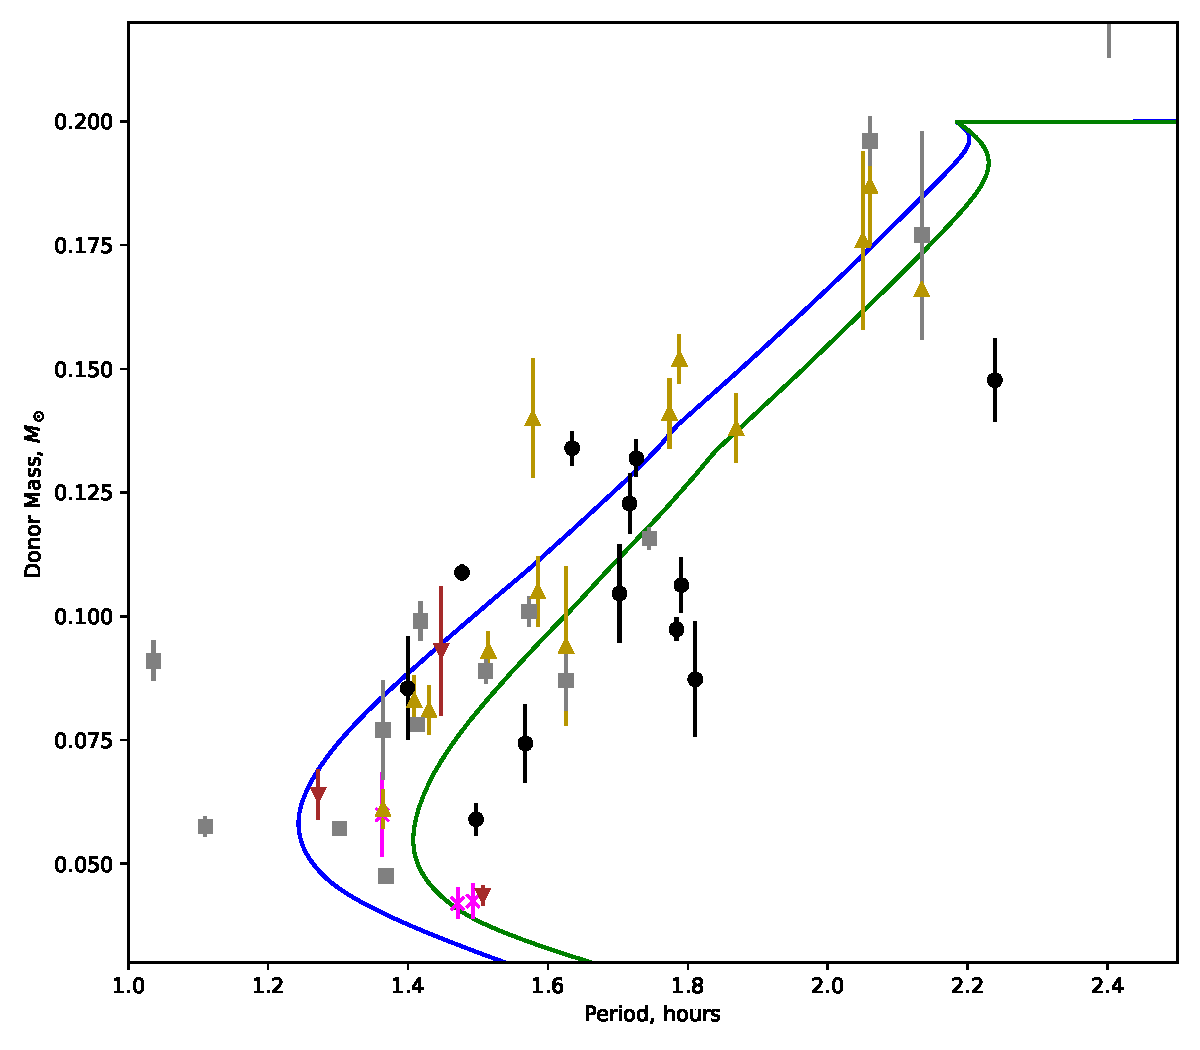
\includegraphics[width=\textwidth]{figures/results/Mdot/K11_donor_track_with_eclipse_modelled_data.pdf}
    \caption{Showing how eclipse modelled observations compare with evolutionary models. The {\bf solid blue line} is the `standard' MESA CV donor track, and the {\bf solid green line} is the `optimal' track, described in \S\ref{sect:results:reproducing K11 tracks}. The {\bf black data with errors} are observations: {\bf circles} are the 3 CVs with peculiar colours from Chapter~\ref{chpt:results:three peculiar white dwarfs}, {\bf crosses} are the 12 systems of Chapter~\ref{chpt:results:characterisation of 12 new CVs}, and {\bf triangles} are data from \citet{McAllister2019}, and {\bf squares} are from \citet{Savoury2011}.}
    \label{fig:discussion:donor model with eclipsers plotted}
\end{figure}

\todo{eCAML instability plot could be made, with the new data added to it}
\todo{The K11 mass-radius relation can be updated? Not really worth it...}



\newpage
\subsection{A preliminary exploration of AML in CVs}
\label{sect:discussion AML}

The original results and analysis of the three CVs in Chapter~\ref{chpt:results:three peculiar white dwarfs} pre-dates the more fully developed method to infer a donor mass loss rate described in \S\ref{sect:modelling:optimising mass loss rate to observations}. An early version of that approach was applied to these systems, and the population of well-characterised CVs that was available at publication. That work is reproduced here, and extended to include the further 12 CVs characterised since this publication.

In order to qualitatively evaluate missing AML, the period \textit{excess} was examined, $P_{\rm ex} = P_{\rm obs} - P_{\rm std}$, where $P_{\rm std}$ is the period predicted by the MESA CV donor track with only $1\times$ gravitational braking below the period gap, interpolated across $M_{\rm donor}$. $P_{\rm obs}$ is the observed period.
To determine $P_{\rm ex}$ from an estimate of $P_{\rm obs}, M_{\rm donor}$, mass samples are drawn from a Gaussian distribution based on the observed mean and standard deviation of $M_{\rm donor}$, and period is interpolated from the evolutionary tracks to give a corresponding $P_{\rm model}$ distribution. As $P_{\rm model}$ is very sensitive to $M_{\rm donor}$, the $P_{\rm model}$ error dominates the uncertainty in $P_{\rm ex}$.
A positive $P_{\rm ex}$ indicates that the model is missing AML, and a negative $P_{\rm ex}$ indicates a model that has too much AML, relative to an observation.

The validity of $P_{\rm ex}$ is vulnerable on two key systematic biases; the validity of $P_{\rm model}$, and the inherent physical variation of the CV population. This is the secondary motivation for the development of the more rigorous methodology of \S\ref{sect:modelling:optimising mass loss rate to observations}, with the primary motivation being the qualitative nature of this approach.

CVs may follow inherently different evolutionary tracks due to differences in donor metallicity \citep{stehle1997, harrison2016}, white dwarf mass \citep{knigge2006}, and the age of the donor when it first contacts the Roche lobe \citep{howell2001}. A population-wide scatter in this parameter space is not captured in the \citet{knigge11} model, which uses fixed values for these variables, but justification for the adopted values are given \citep{knigge11, knigge2006}.
If any individual system deviates from the adopted values in the models of \citet{knigge11} then $P_{\rm ex}$ for that system will be influenced by these differences as well as any extra AML. However, conclusions about $P_{\rm ex}$ drawn from the population at large should remain robust, as long as the population doesn't differ systematically from the values adopted in the models. The white dwarf mass used by \citet{knigge11} is somewhat lower than more recent observations suggest, using $M_{\rm WD} = 0.75 M_\odot$ versus the more recent value of $M_{\rm WD} = 0.83 \pm 0.17 M_\odot$ \citep{pala2020}. Modelling will be necessary to properly characterise the effect of this change on the donor evolutionary tracks, as this will affect both the size of the Roche lobes, and the rate of gravitational wave AML. However, other CV models suggest that the effect will be small; at most around 2 minutes \citep{goliasch2015}.

More seriously, $P_{\rm ex}$ is only an accurate proxy of additional AML if the underlying donor physics in the model are correct. For example, if the models incorrectly predict the mass of systems in the period gap, this can have a large effect on $P_{\rm ex}$. In the models of \citet{knigge11} this mass is fixed at the empirically derived value of $0.2 M_\odot$, as observations of superhumping and eclipsing CVs suggest that period gap occurs at donor masses of $0.20 \pm 0.02 M_\odot$ \citep{knigge2006}. Using model tracks with lower or higher masses for the donor mass of the period gap would alter $P_{\rm ex}$, though in this case the broad trend in $P_{\rm ex}$ will again be unchanged.

The result is plotted in Figure~\ref{fig:period excess}. These data are fit with a straight line, and as the data have significant uncertainty in both axes, the sum orthogonal distance from the data is minimised to find the best fit \citep{hogg2010}. The best-fit lines to the two data sets are $P_{\rm ex} = -(2.97\pm0.99) M_{\rm donor} + (0.34\pm0.09)$ and $P_{\rm ex} = -(1.66\pm0.32) M_{\rm wd} + (1.30\pm0.24)$.
I find that the best-fit to $P_{\rm ex}$ as a function of both $M_{\rm donor}$ and $M_{\rm wd}$ to be significant: $\sim 5\sigma$ from the null hypothesis of 0 in the case of $M_{\rm wd}$, and $\sim 3\sigma$ for $M_{\rm donor}$.
 However, note that the best-fit line for $M_{\rm donor}$ does \textit{not} pass through $P_{\rm ex} = 0$ at $M_{\rm donor} = 0.20 M_\odot$ as expected, unless the $3\sigma$ confidence on the gradient and intercept are considered.

Again, it is stressed that the only robust product of this analysis is the \textit{sign of the gradient} of the $M - P_{\rm ex}$ relationship, and that its steepness and y-intercept are both subject to systematic errors that are not captured in the statistical errors given above. Despite this, the clear and statistically significant increase in $P_{\rm ex}$ towards low masses implies that additional AML has a larger effect on the donor at low masses.

Note that $P_{\rm ex}$ considers a changing gravitational braking strength, which declines as the total system mass falls.
There are then three cases to describe the trend in $P_{\rm ex}$: the excess AML also declines in strength but more slowly than gravitational losses; excess AML is roughly constant across the range of $M_{\rm donor}$ or $M_{\rm wd}$; or excess AML actually increases in strength towards lower $M_{\rm donor}$ or $M_{\rm wd}$. Note that none of these options translate to the ``optimal'' \citet{knigge11} models which adopt additional AML of the same form as GWB, but are compatible with the eCAML solution for excess AML.


\begin{figure}
    \centering
    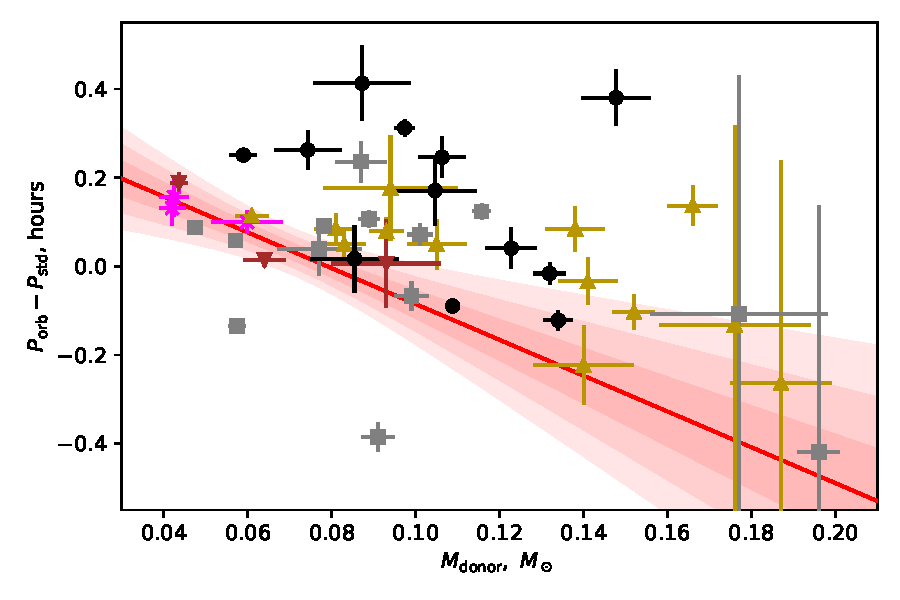
\includegraphics[width=\columnwidth]{figures/results/Mdot/Period_excess_Mr.pdf}
    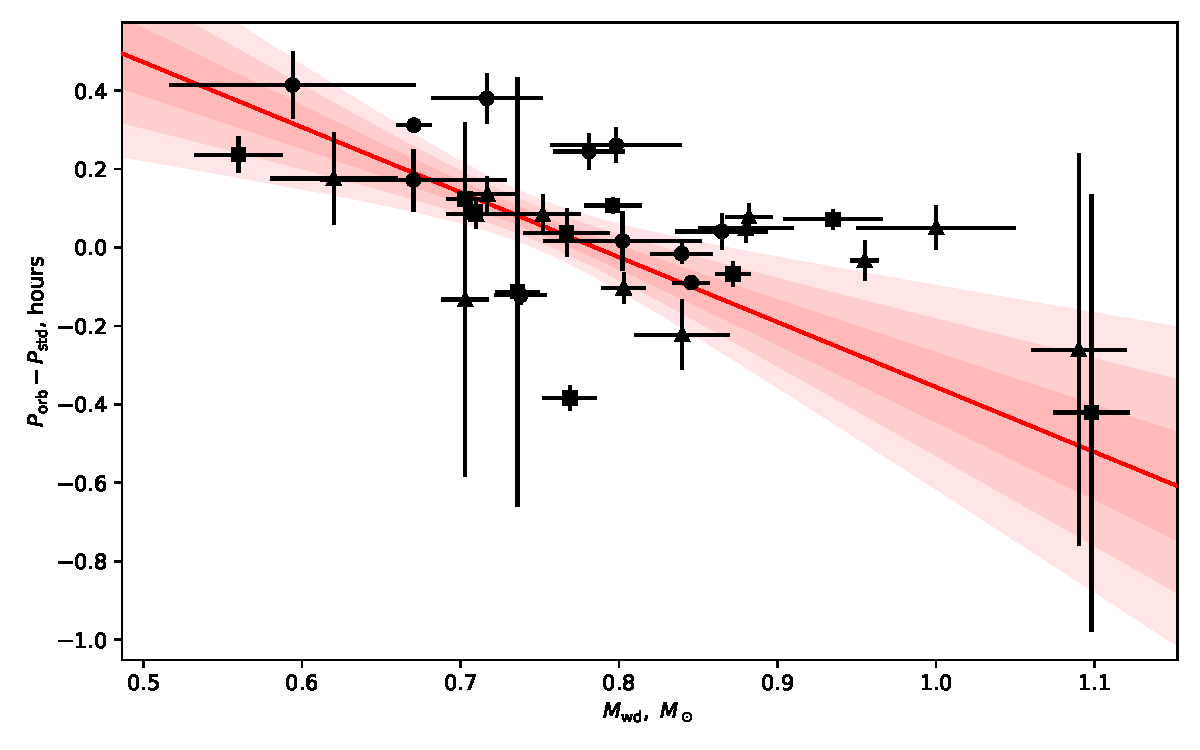
\includegraphics[width=\columnwidth]{figures/results/Mdot/Period_excess_Mwd.pdf}
    \caption{The relation between the two body masses, and the period excess, $P_{\rm ex}$ is shown. The {\rm black crosses with error bars} are the observed data, and the {\bf solid red line} shows the best-fit solution to the data. {\bf Shaded red regions} show successively lower confidence intervals, with the darkest region being $1\sigma$ confidence, and the lightest region being $3\sigma$ confidence. The lines of best fit have the forms: $P_{\rm ex} = -(2.97\pm0.99) M_{\rm donor} + (0.34\pm0.09)$ and $P_{\rm ex} = -(1.66\pm0.32) M_{\rm wd} + (1.30\pm0.24)$.}
    \label{fig:period excess}
\end{figure}
% \begin{figure}
%     \centering
%     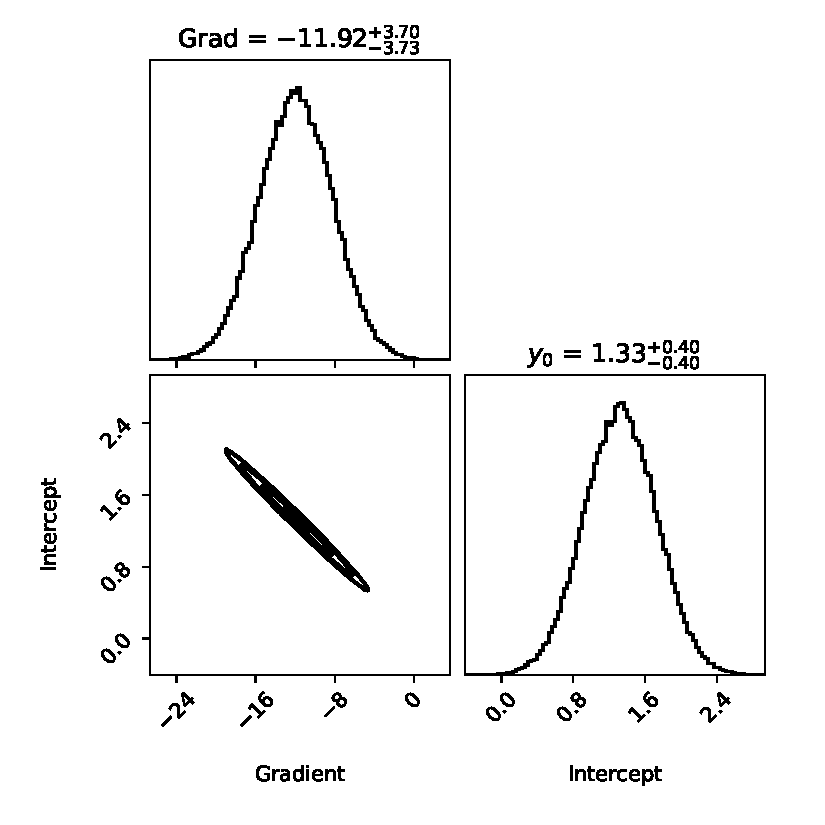
\includegraphics[width=\columnwidth]{figures/results/Mdot/Period_excess_Mr_corner.pdf}
%     \caption{Showing the distribution of the best fit to the $M_{\rm donor} - P_{\rm ex}$ relationship plotted in the top panel of Figure~\ref{fig:period excess}.}
%     \label{fig:period excess donor_corner}
% \end{figure}
% \begin{figure}
%     \centering
%     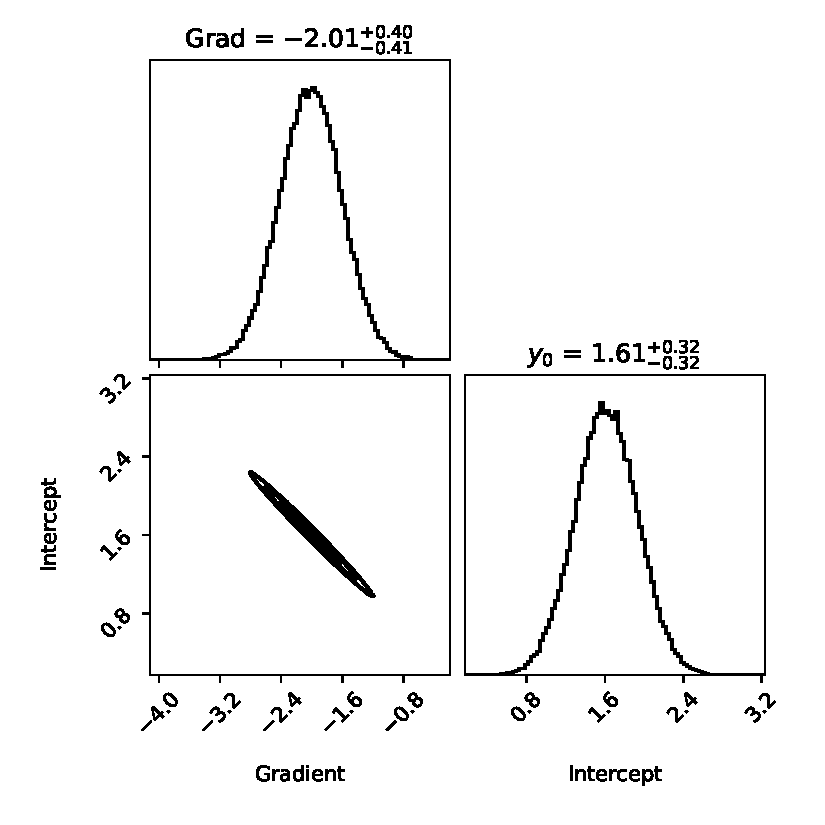
\includegraphics[width=\columnwidth]{figures/results/Mdot/Period_excess_Mwd_corner.pdf}
%     \caption{Showing the distribution of the best fit to the $M_{\rm wd} - P_{\rm ex}$ relationship plotted in the bottom panel of Figure~\ref{fig:period excess}.}
%     \label{fig:period excess white dwarf corner}
% \end{figure}


\section{Inferring mass loss rate from donor properties}
\label{sect:discussion:evolutionary modelling}

First, I compare the mass loss rates of the donor inferred from donor properties, with the mass loss rates inferred from the white dwarf properties. Figure~\ref{fig:discussion:compare Mdot from donor and WD} plots the $\dot M$ from each method, and two differences between the data are immediately obvious: the white dwarf properties consistently indicate a higher $\dot M$, and using the donor properties results in significantly larger uncertainties.

The white dwarf indicating a higher mass loss rate is expected, as recent dwarf novae (a.k.a periods of intense accretion onto the white dwarf) cause the surface to heat up, but after a dwarf nova has subsided the white dwarf will take hundreds to tens of thousands of years to adjust to the lower accretion rate.
Several of the CVs in this sample were identified for eclipse modelling follow-up \textit{specifically} based on observations of recent outbursts, so it is unsurprising that the white dwarf can indicate $\dot M$ an order of magnitude higher than the donor does. As the white dwarf is subject to inflation by these short-term variations, the donor-based method is considered more reliable for the long-term $\dot M$ baseline and hereafter when values of $\dot M$ are used, they are the values derived from the donor properties.
\begin{figure}
    \centering
    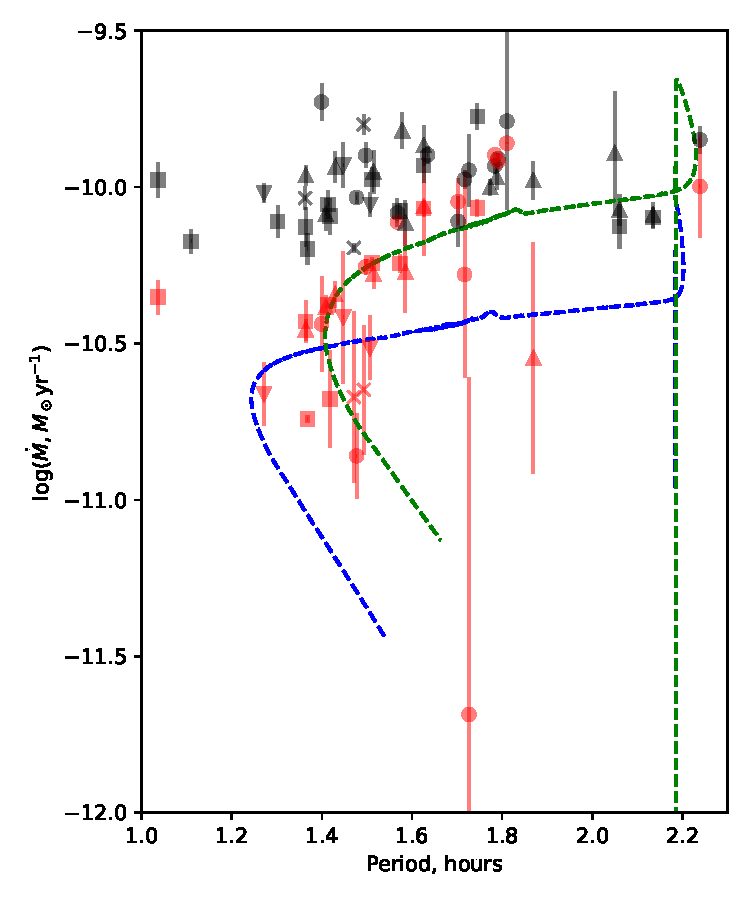
\includegraphics[width=\textwidth]{figures/results/Mdot/compare_mdot_from_donor_vs_wd_vs_period.pdf}
    \caption{Comparing the mass loss rates inferred from the donor properties ({\bf red crosses}) with those inferred from the white dwarf properties ({\bf blue crosses}).}
    \label{fig:discussion:compare Mdot from donor and WD}
\end{figure}

It is interesting to compare the correlation between the mass loss rate and the masses of the two bodies in a CV.

Recall from the discussion in \S\ref{sect:introduction:magnetic braking} that, if the missing AML from CV models is rooted in residual magnetic braking, {\it and these prescriptions for magnetism are accurate}, we would expect to see a correlation between $M_{\rm donor}$ and $\dot M$.
This is because both prescriptions are dependent on the Rossby number, a function of the rotational period, which itself is a function of donor mass in this mass range.
If, however, the CAML model is correct and the source of the missing AML is the white dwarf's ejecta carrying momentum with it from the system (refer to \S\ref{sect:introduction:CAML}), we would expect a correlation between $M_{\rm wd}$ and $\dot M$, as a lower total system mass would allow material to leave with a higher velocity, and the white dwarf dominates the total mass of a CV.
Of course, the two sources of extra AML are not mutually exclusive, and may co-exist.

To probe for these correlations the $\chi^2$ test is insufficient, since both axes have significant errors.
Rather, the minimised quantity is the sum of the squared orthogonal distances between the observations and a proposed best-fit line, weighted by error. Python's \lstinline{scipy} package, \lstinline{ODR} was used to perform this fitting.

Figure~\ref{fig:discussion:donor mass vs Mdot fit} shows the best fit line for $\dot M(M_{\rm donor})$, and Figure~\ref{fig:discussion:white dwarf mass vs Mdot fit} is the fit for $\dot M(M_{\rm wd})$.

These figures show a correlation in each case. Lower $M_{\rm wd}$ appear to correlate with \textit{higher} $\dot M$, and lower $M_{\rm donor}$ appear to correlate with \textit{lower} $\dot M$.
The correlation between $M_{\rm wd}$ and $\dot M$, is reasonably confident -- the est-fit gradient is $4.5\sigma$ from the null-hypothesis of 0.
However, the $M_{\rm donor}$ case is comparable, with a best-fit gradient $4.4 \sigma$ from 0.
% Therefore, we can consider these findings as preliminary evidence for a co-existence between a small degree of residual magnetic braking below the period gap, \textit{and} an excess AML over gravitational wave braking that is due to CAML.

There are a few factors to consider when deciding how convincing these findings are.
The sample size is still small, only 25 systems, and the errors on $\dot M$ are large. Further, there may be a problem with systematic error -- it may that this sample is biased towards CVs with more excess AML, as these would be more inflated and thus less likely to be smaller than the Brown relation suggests for a zero-$\dot M$ star.
A more robust understanding of the low-mass main sequence mass-radius relation is crucial to a more confident re-analysis of these results.

\begin{figure}
    \centering
    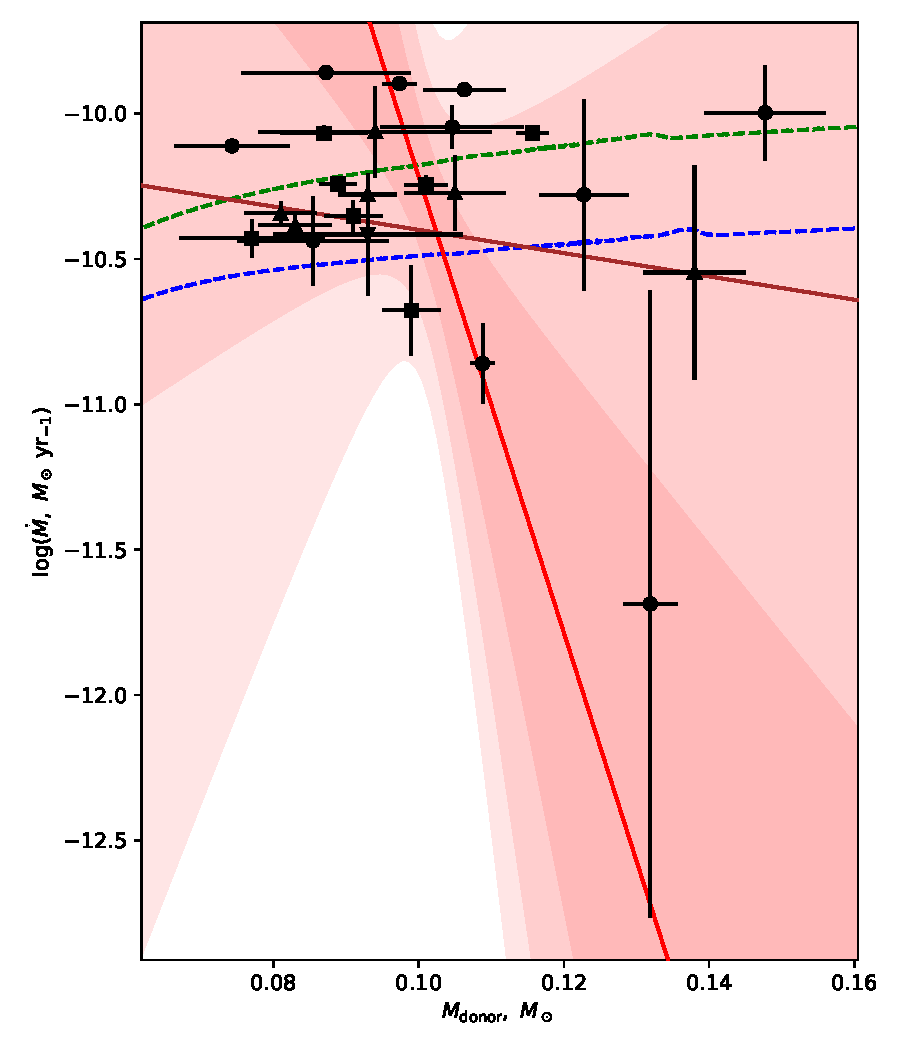
\includegraphics[width=\textwidth]{figures/results/Mdot/Mr_Mdot.pdf}
    \caption{Showing the correlation between the donor mass and mass loss rate. The {\bf black crosses with error bars} show the observations, and the {\bf red line} shows the best fit to the data, with the {\bf shaded red region} showing the coverage of the uncertainty in the line parameters. The darkest region is $1\sigma$, the middle region is $2\sigma$, and the lightest region shows $3\sigma$. The {\bf dashed blue line} shows the value predicted by the `standard' MESA CV model, and the {\bf dashed green line} is the `optimal' MESA CV track. The best fit line has the form $\log (\dot M,\ M_\odot\ {\rm yr}^{-1}) = (19.61\pm4.50) (M_{\rm donor}, M_\odot) - (12.02\pm0.42)$. }
    \label{fig:discussion:donor mass vs Mdot fit}
\end{figure}
% \begin{figure}
%     \centering
%     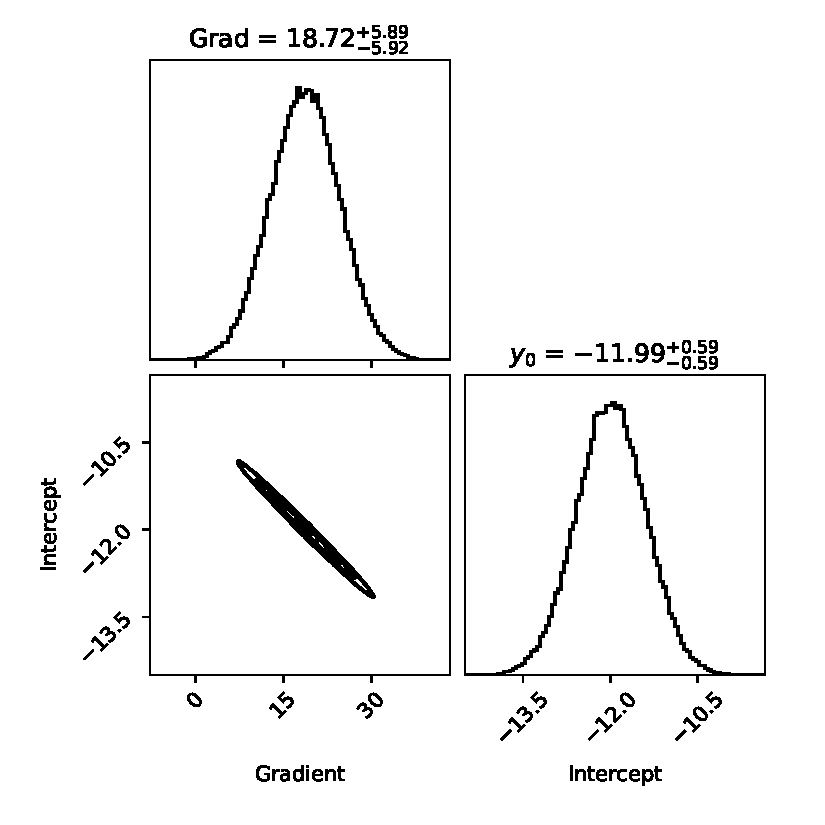
\includegraphics[width=\textwidth]{figures/results/Mdot/Mr_Mdot_corner.pdf}
%     \caption{Showing the posterior distributions of the gradient and intercept of the best fit line in Figure~\ref{fig:discussion:donor mass vs Mdot fit}.}
%     \label{fig:discussion:donor mass vs Mdot corner}
% \end{figure}
\begin{figure}
    \centering
    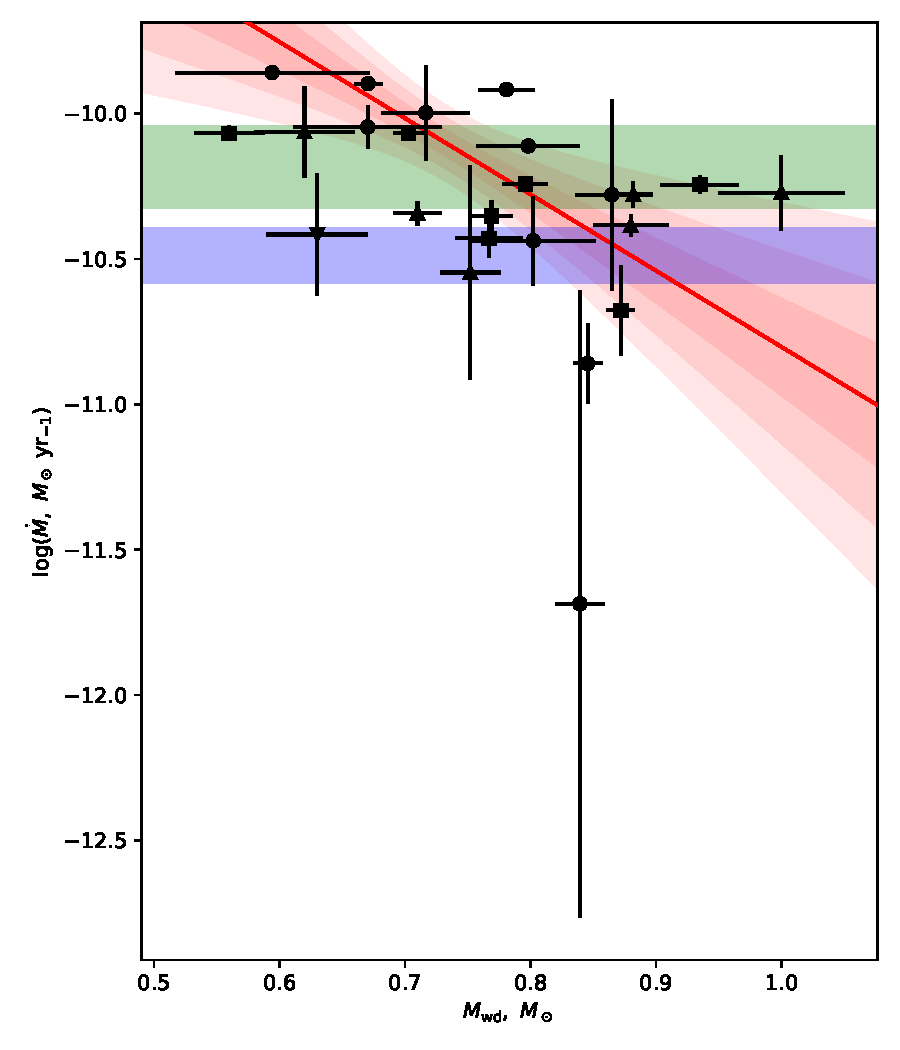
\includegraphics[width=\textwidth]{figures/results/Mdot/Mwd_Mdot.pdf}
    \caption{Showing the correlation between the white dwarf mass and mass loss rate. Symbols are similar to Figure~\ref{fig:discussion:donor mass vs Mdot fit}, though here the range of values predicted by the `standard' and `optimal' MESA CV models are shown as the {\bf blue shaded region} and {\bf green shaded region}, respectively. The best fit line has the form $\log ( \dot M,\ M_\odot\ {\rm yr}^{-1}) = (-2.27 \pm 0.50) (M_{\rm donor}, M_\odot) - (8.48 \pm 0.36)$}
    \label{fig:discussion:white dwarf mass vs Mdot fit}
\end{figure}
% \begin{figure}
%     \centering
%     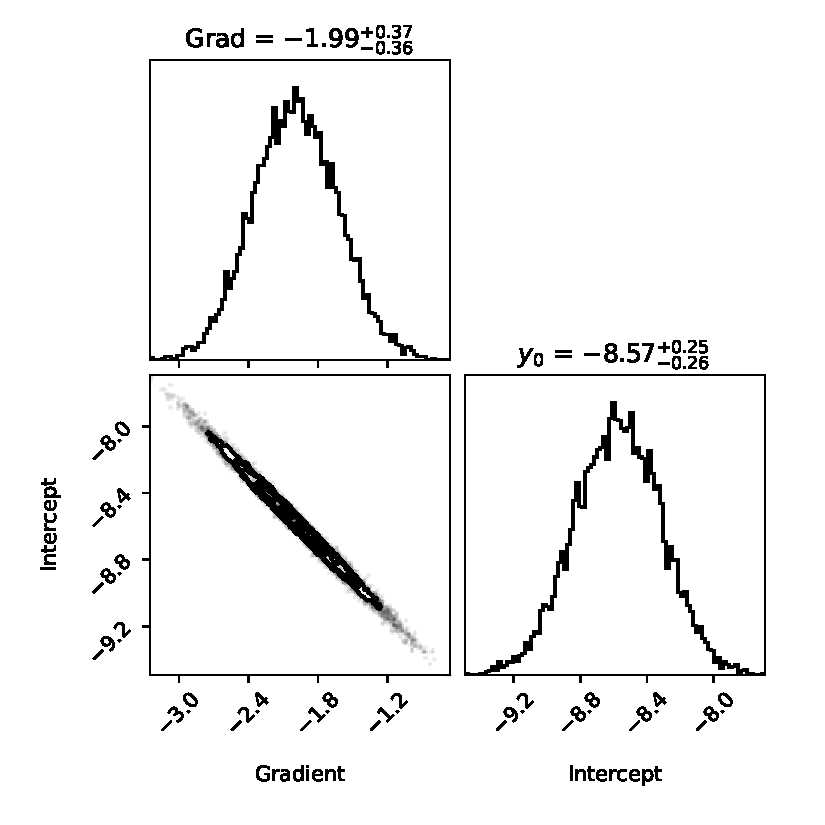
\includegraphics[width=\textwidth]{figures/results/Mdot/Mwd_Mdot_corner.pdf}
%     \caption{Showing the posterior distributions of the gradient and intercept of the best fit line in Figure~\ref{fig:discussion:white dwarf mass vs Mdot fit}.}
%     \label{fig:discussion:white dwarf mass vs Mdot corner}
% \end{figure}


It is possible to more directly probe the AML of the CVs -- Equation~\ref{eqn:modelling:Jdot from Mdot} shows how the AML can be calculated from $M_{\rm wd},\ M_{\rm donor},\ \dot M$, and $a$.
Figures~\ref{fig:discussion:donor mass vs Jdot fit}~and~\ref{fig:discussion:white dwarf mass vs Jdot fit} show the best-fit to the $\dot J$ \textit{excess}, which has had the $\dot J_{\rm GR}$ predicted by MESA at the appropriate donor mass ($\dot J_{\rm MESA}$) subtracted.
Again, the correlation with $M_{\rm wd}$ is reasonably significant at $4.1\sigma$ from a gradient of 0, but here the donor correlation is less significant at $3.4\sigma$, though this is more significant than in the case of $\dot M$.
\begin{figure}
    \centering
    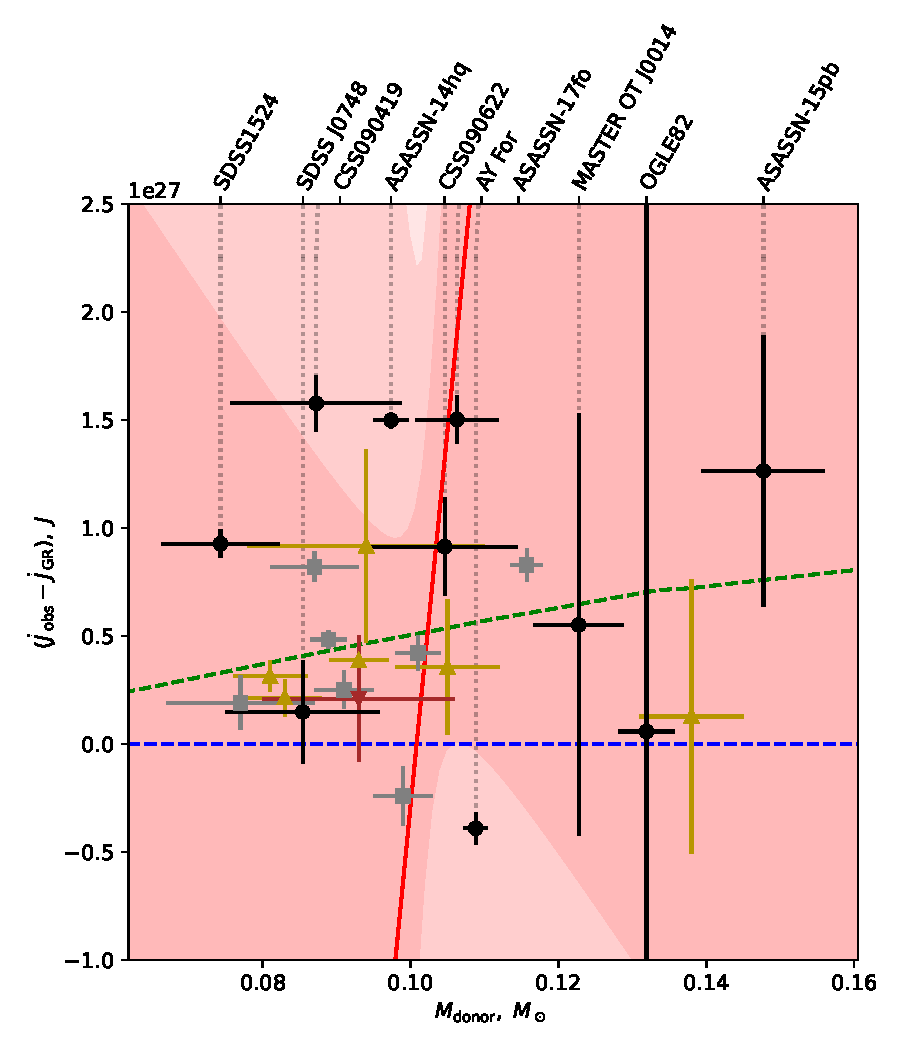
\includegraphics[width=\textwidth]{figures/results/Mdot/Mr_Jdot_ex.pdf}
    \caption{Showing the correlation between the donor mass and angular momentum loss rate, $\dot J$. Symbols are similar to Figure~\ref{fig:discussion:donor mass vs Mdot fit}, though here the {\bf dashed blue line} shows perfect agreement between observations and gravitational angular momentum loss. Note that the two data with vertical errors spanning the full height of the plot extend by approximately an order of magnitude in each direction, but are truncated for clarity. The line of best fit has the form $(\dot J_{\rm obs} - \dot J_{\rm MESA}), J = (2.68\pm0.79) \times 10^{28}(M_{\rm donor}, M_\odot) - (2.17\pm0.71)\times10^{27}$}
    \label{fig:discussion:donor mass vs Jdot fit}
\end{figure}
% \begin{figure}
%     \centering
%     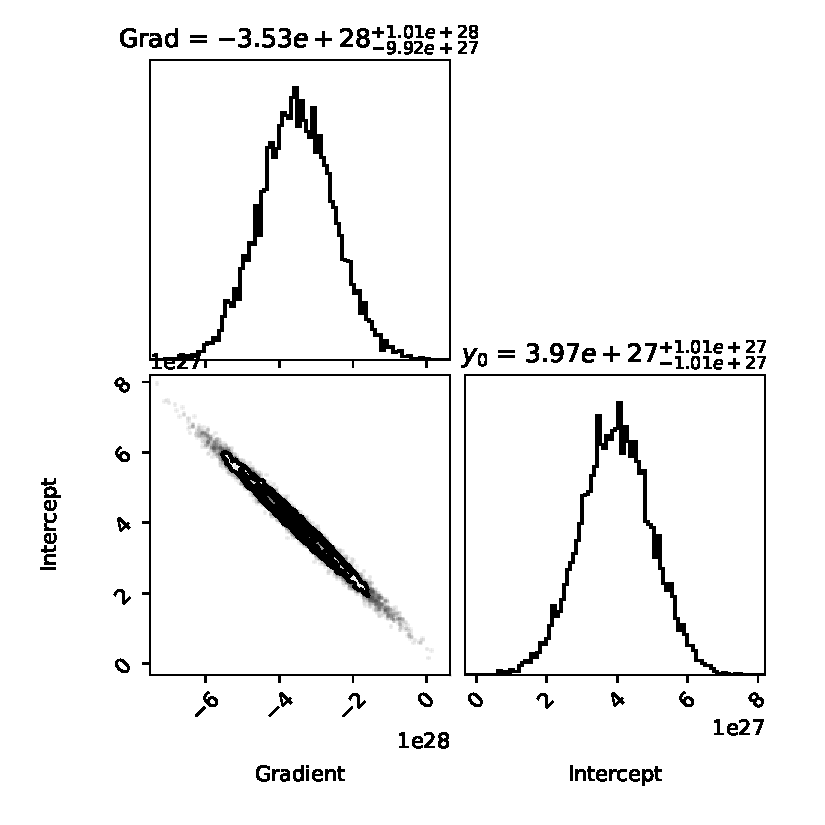
\includegraphics[width=\textwidth]{figures/results/Mdot/Mr_Jdot_ex_corner.pdf}
%     \caption{Showing the posterior distributions of the gradient and intercept of the best fit line in Figure~\ref{fig:discussion:donor mass vs Jdot fit}.}
%     \label{fig:discussion:donor mass vs Jdot corner}
% \end{figure}

\begin{figure}
    \centering
    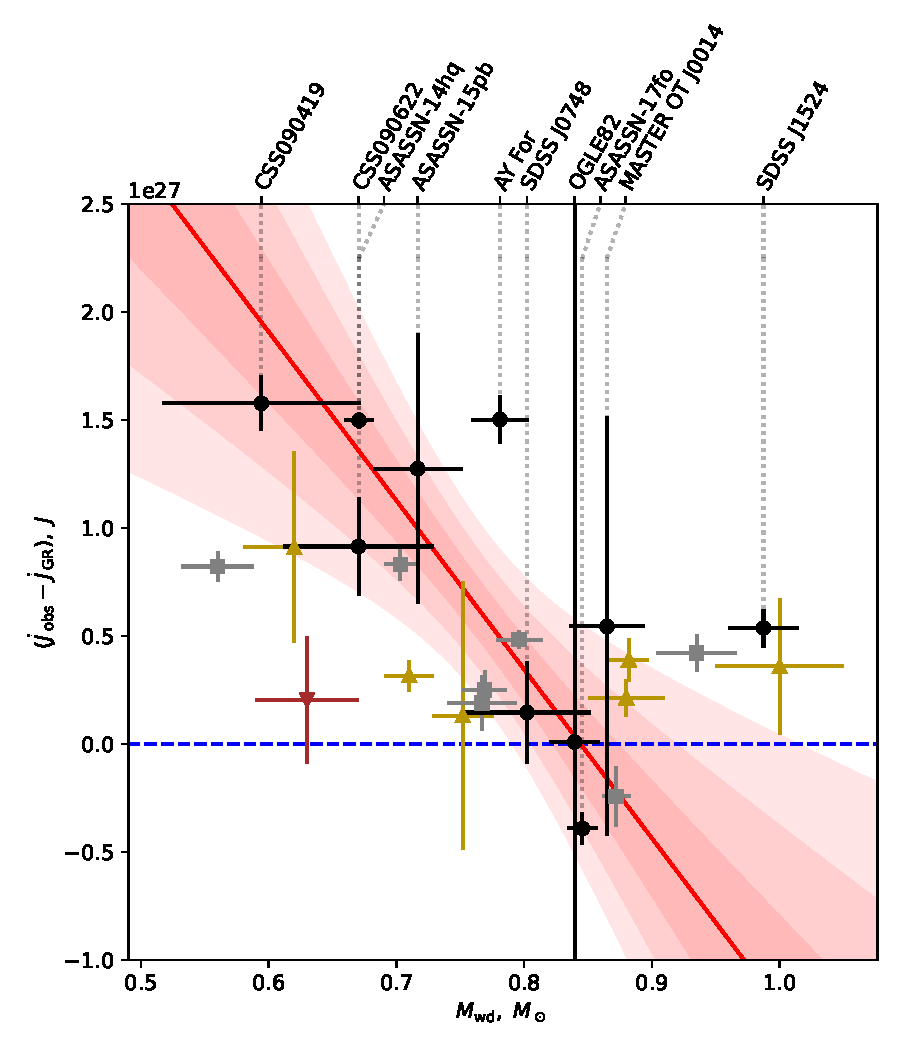
\includegraphics[width=\textwidth]{figures/results/Mdot/Mwd_Jdot_ex.pdf}
    \caption{Showing the correlation between the white dwarf mass and angular momentum loss rate, $\dot J$. Symbols are similar to Figure~\ref{fig:discussion:white dwarf mass vs Jdot fit}, and the best fit line has the form $(\dot J_{\rm obs} - \dot J_{\rm MESA}), J = -(3.62\pm0.89) \times 10^{27}(M_{\rm donor}, M_\odot) - (2.98\pm0.67)\times10^{27}$}
    \label{fig:discussion:white dwarf mass vs Jdot fit}
\end{figure}
% \begin{figure}
%     \centering
%     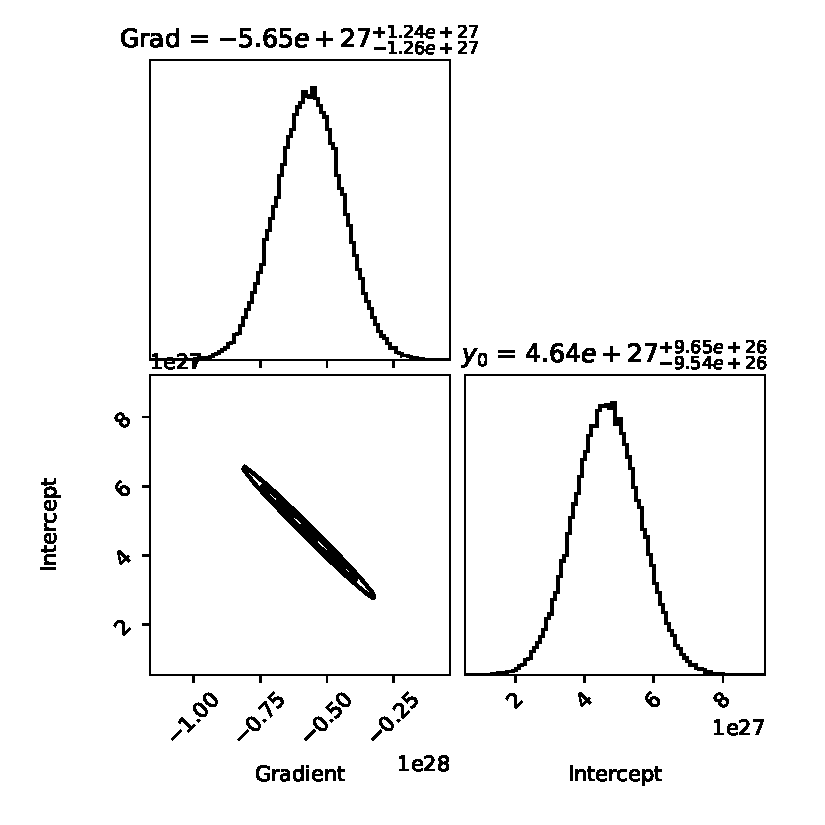
\includegraphics[width=\textwidth]{figures/results/Mdot/Mwd_Jdot_ex_corner.pdf}
%     \caption{Showing the posterior distributions of the gradient and intercept of the best fit line in Figure~\ref{fig:discussion:white dwarf mass vs Jdot fit}.}
%     \label{fig:discussion:white dwarf mass vs Jdot corner}
% \end{figure}


Three possibilities for the form of excess AML were suggested in \S\ref{sect:discussion AML}: the excess AML also declines in strength but more slowly than gravitational losses; excess AML is roughly constant across the range of $M_{\rm donor}$ or $M_{\rm donor}$; or excess AML increases in strength towards lower $M_{\rm donor}$ or $M_{\rm wd}$.
We can now see that the excess AML appears to increase in strength towards lower component masses.

Based on the analysis above, it appears that both residual magnetic braking and eCAML have some influence on the evolution of a short period CV, with there being consistent signs of increasing excess AML towards both lower donor masses, and lower white dwarf masses.
% We can now discriminate between these with the quantitative analysis given here, and see that the degree of excess AML is most likely to be a negative correlation with $M_{\rm wd}$, in line with the CAML model of CVs.
As a final test of eCAML, the stability plot given in Figure~\ref{fig:introduction:Schreiber 2016 figure 2} can be augmented to include the new CVs of this work, from which we can see that no CVs exist outside of the stability region.
\todo{Make the eCAML plot with the new data.}

Further work is needed to grow the population of eclipse modelled low-$M_{\rm donor}$ CVs and improve these statistics, and continued eclipse modelling targeting short period CVs will be valuable to determining the probable source of excess AML.
Specific effort should be targeted towards confident characterisation of CVs at higher $M_{\rm donor}$ of $\sim0.15$, where existing data have large error bars. The clustering of confident data at lower masses leaves the current sample prone to poor extrapolation beyond $\sim 0.11 M_\odot$.
However, lending credence to these results is the consistency with findings of \citet{Pala2021}, who used the white dwarf properties to arrive at a similar conclusion.

\todo{Augment MESA to include my new AML prescription, and run it!}